\documentclass{article}
\usepackage[T1]{fontenc}
\usepackage{lmodern}
\usepackage{graphicx}
\usepackage{amsmath,amssymb}
\usepackage[a4paper,margin=2cm]{geometry}
\usepackage[absolute,overlay]{textpos}
\setlength{\TPHorizModule}{1mm}
\setlength{\TPVertModule}{1mm}
\usepackage[indonesian]{babel}
\usepackage{hyperref}
\setlength{\emergencystretch}{2em}
% unit: Halaman 5

\begin{document}

% === Halaman 5 (llm) ===

\vspace{103.65mm}

Client
\vspace{50mm}
Browser

% deskripsi: Diagram yang mengilustrasikan siklus permintaan dan tanggapan HTTP antara Client (Browser) dan Server, menunjukkan panah aliran 'HTTP Request' dari client ke server dan 'HTTP Response' dari server kembali ke client.
% bbox normalisasi: [0.2520, 0.2710, 0.6810, 0.6200]
\begin{textblock*}{90.09mm}(52.92mm,80.49mm)
\noindent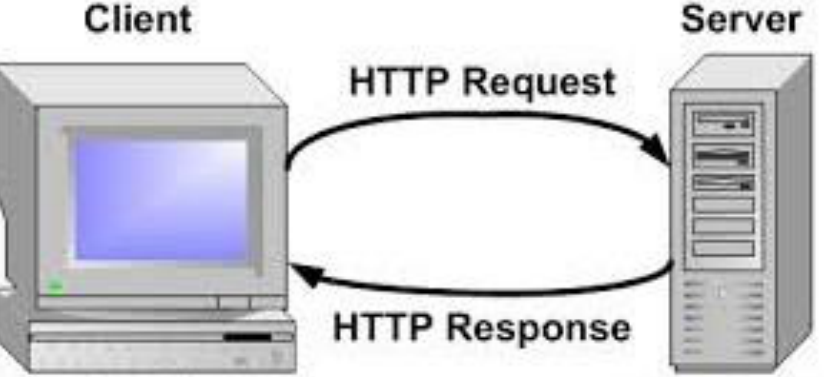
\includegraphics[width=90.09mm,height=103.65mm]{../../images/llm/page_005_img_01.png}%
\end{textblock*}

\end{document}
